
\documentclass[ms.tex]{subfiles}
\begin{document}

\section{Predicted SN Ia Rates}
\label{sec:predictions}

% fig 2
\begin{figure*}
\centering
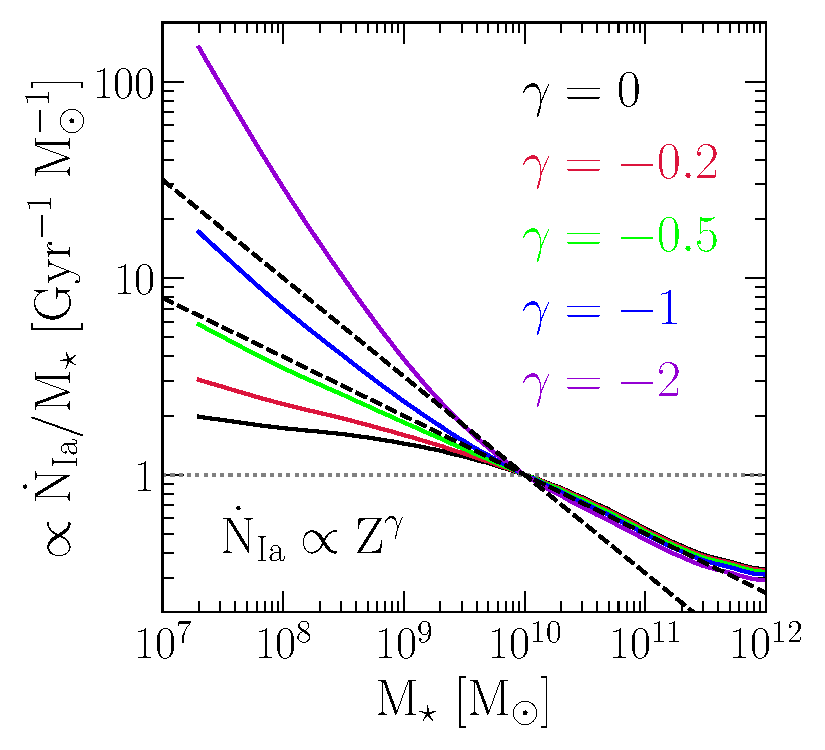
\includegraphics[scale = 0.55]{umachine_iarate_metdep.pdf}
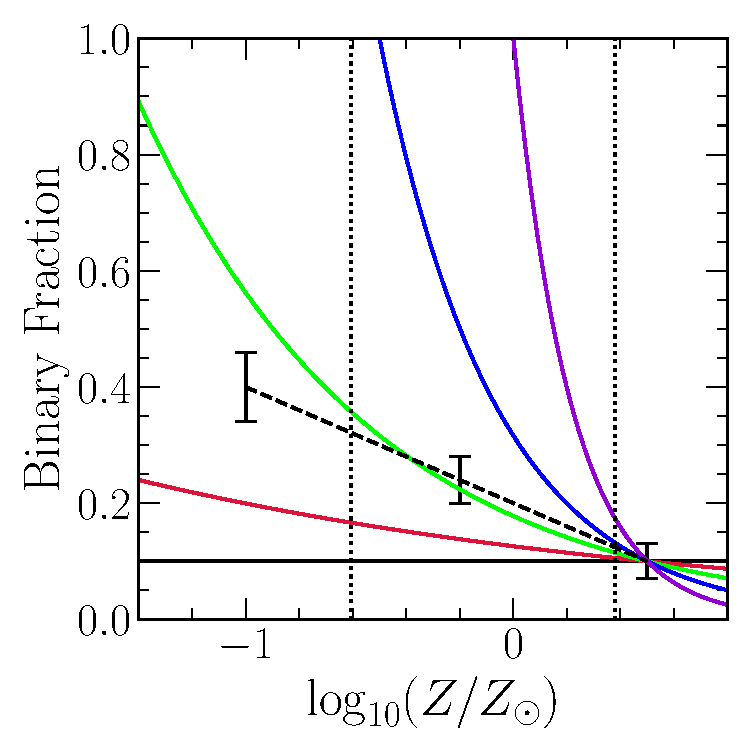
\includegraphics[scale = 0.56]{binaries_zscaling.pdf}
\caption{
\textbf{Left}: Theoretically predicted scalings of the specific SN Ia rate with
galaxy stellar mass (see equation~\ref{eq:specia}) assuming the mean SFHs
reported by~\um~and a single power-law dependence on metallicity~$Z^\gamma$
with~$\gamma = 0$ (i.e. no dependence; black),~$\gamma = -0.2$ (red),
$\gamma = -0.5$ (green),~$\gamma = -1$ (blue), and~$\gamma = -2$ (purple).
Following~\citet{Brown2019} and~\citet{Gandhi2022}, we normalize all rates to
a value of 1 at~$\mstar = 10^{10}~\msun$.
\textbf{Right}: The same metallicity scalings as in the left panel in
comparison to the close binary fractions observed in APOGEE
\citep[][black dashed line with error bars]{Moe2019}.
All metallicity scalings are normalized to the observed binary fraction of 10\%
at~$\log_{10}(Z / Z_\odot) = +0.5$.
We mark the characteristic metallicity of a~$\mstar = 10^{7.2}~\msun$ galaxy
($\log_{10}(Z / Z_\odot) \approx -0.6$) according to the~\citet{Zahid2014} MZR
with a black dotted line.
}
\label{fig:specia_metdep}
\end{figure*}

The left panel of Fig.~\ref{fig:specia_metdep} shows the specific SN Ia rate
as a function of~$\gamma$ in comparison to the~$\dot{\text{N}}_\text{Ia} /
\mstar \sim \mstar^{-0.5}$ and~$\dot{\text{N}}_\text{Ia} / \mstar \sim
\mstar^{-0.3}$ scalings of the observed rate with the~\citet{Bell2003} and
\citet{Baldry2012} SMFS, respectively.
The metallicity dependence has a significant impact only below
$\mstar \approx 3\times10^9~\msun$ due to the shape of the MZR;
this is the mass above which the MZR flattens considerably (see
Fig.~\ref{fig:sfh_mzr}).
Assuming no metallicity dependence (i.e.~$\gamma = 0$), these calculations
suggest that the variations in SFHs between~$\sim$$10^{7.2}$ and
$\sim$$10^{10}~\msun$ can account for only a factor of~$\sim$2 increase in the
specific SN Ia rate.
The~$\gamma = -0.5$ case is generally consistent with a mass dependence
of~$\mstar^{-0.3}$, while the steeper dependence of~$\mstar^{-0.5}$ would
require a stronger scaling of roughly~$\gamma \approx -1.5$.
% \citet{Gandhi2022} advocate for a~$\gamma \approx -0.5$ scaling, additionally
% demonstrating that incorporating this metallicity dependence into the
% FIRE-2\footnote{
% 	Feedback In Realistic Environments.
% 	\url{https://fire.northwestern.edu/}
% } cosmological zoom-in simulations~\citep{Hopkins2018} leads to better
% agreement with the stellar masses and iron abundances measured by
% \citet{Gallazzi2005} and~\citet{Kirby2013}.
\par
In the right panel of Fig.~\ref{fig:specia_metdep}, we compare the same
scalings to the close binary fractions in APOGEE measured by~\citet{Moe2019}.
The line at~$Z \approx 10^{-0.6} Z_\odot$ is the characteristic abundance of
an~$\mstar = 10^{7.2}~\msun$ galaxy in the~\citet{Zahid2014} parametrization.
For the range of metallicities spanned by the stellar masses we explore here,
the close binary fraction is remarkably consistent with a~$\gamma = -0.5$
scaling with metallicity.
% If the~$\sim$$\mstar^{-0.3}$ scaling found by~\citet{Gandhi2022} is accurate,
% then this result suggests that the increase of the specific SN Ia rate with
% decreasing stellar mass can be explained entirely by dwarf galaxies having more
% extended SFHs and a higher close binary fraction due to their lower abundances.
If one instead takes~$Z \approx 0.1Z_\odot$ for a~$\sim$$10^{7.2}~\msun$ galaxy
as suggest by~\citet{Andrews2013}, then there is a slight tension between a
$\gamma = -0.5$ scaling and the close binary fraction measured by
\citet{Moe2019}.
There is some additional freedom to adjust the metallicity dependence beyond
that of binaries, so the agreement need not be perfect.
Any additional increase in the SN Ia rates not supplied by an increased binary
fraction could arise due to more massive WDs forming at low~$Z$ -- the scenario
postuled by~\citet{Kistler2013}.
% If both the~\citet{Andrews2013} MZR and the~$\gamma = -0.5$ scalings are
% accurate, then it would be reasonable to suggest that the additional increase
% in the SN Ia rates not supplied by the increased binary fraction arise due to
% more massive WDs forming at low~$Z$ -- the scenario postulated by
% \citet{Kistler2013}.
Nonetheless, the scaling of the close binary fraction with metallicity can
explain the majority of the effect in this case anyway.
If instead the~$\sim M_\star^{-0.5}$ found by~\citet{Brown2019} is accurate,
then the required~$\gamma \approx -1.5$ scaling cannot be explained by the
close binary fraction alone as it would reach unphysical values ($>1$) within
the range of observed metallicities.
% Such scalings are disfavored by~\citet{Gandhi2022} because they fail to
% reproduce the well-known correlations between stellar [Mg/Fe] and [Fe/H]
% abundances as observed in M31 satellites by~\citep*{Vargas2014} but are still
% within the range of theoretical possibilities because only a small fraction of
% WDs actually explode ($\sim4$\% if the progenitors are~$\sim3 - 8~\msun$
% stars;~\citealp{Maoz2012b}).
% In the next section, we discuss potential observational diagnostics of
% a~$Z^{-0.5}$ metallicity dependence or lack thereof.

% fig 3
\begin{figure*}
\centering
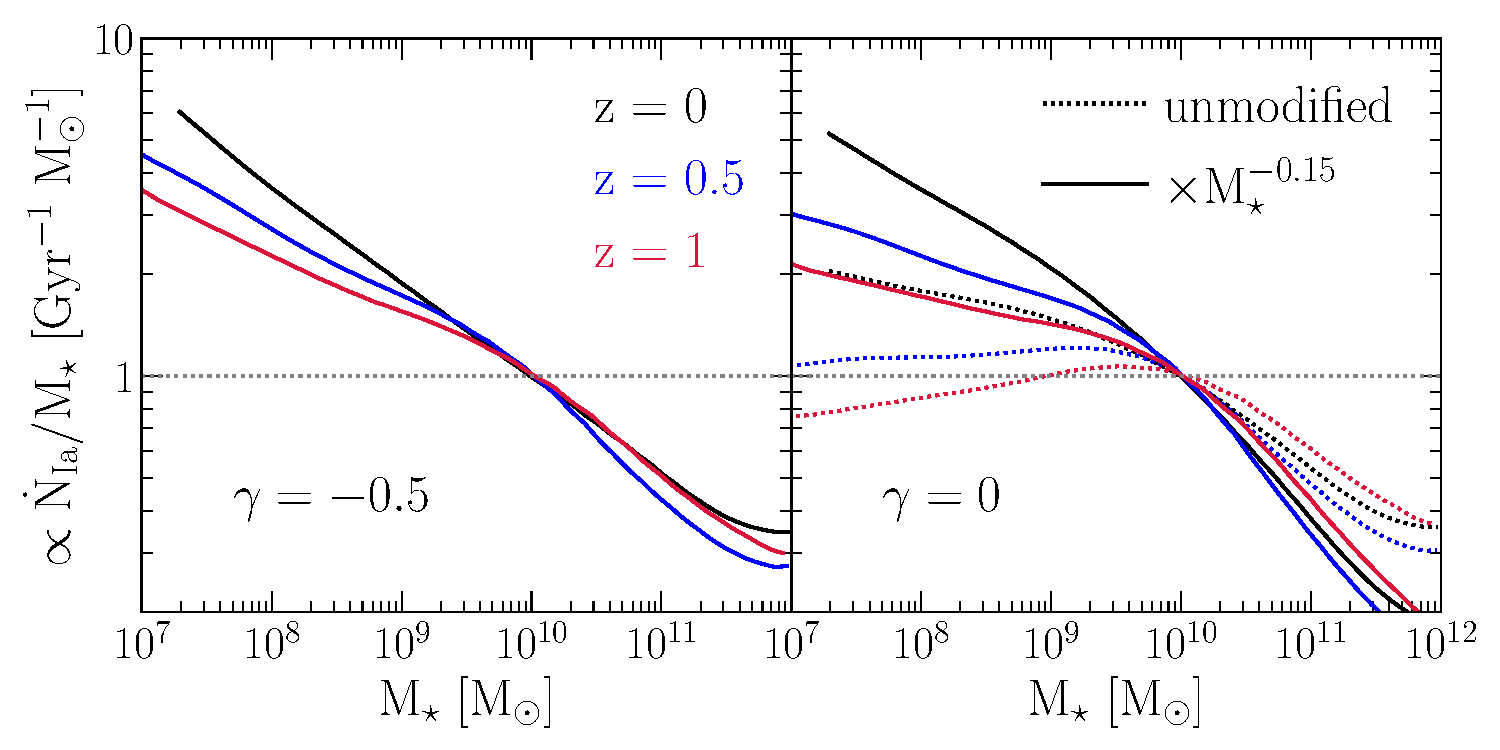
\includegraphics[scale = 0.56]{umachine_iarate_redshiftevol.pdf}
\caption{
The specific SN Ia rate as a function of stellar mass with ($\gamma = -0.5$,
left) and without ($\gamma = 0$, right) a metallicity dependence at redshifts
$z = 0$ (black),~$z = 0.5$ (blue), and~$z = 1$ (red).
Following~\citet{Brown2019} and~\citet{Gandhi2022}, we normalize all rates to
a value of 1 at~$\mstar = 10^{10}~\msun$.
In the right panel, we artificially amplify the rates by a factor of
$(M_\star / 10^{10}~\msun)^{-0.15}$ to bring the~$z = 0$ predictions into
better agreement with an~$\sim M_\star^{-0.3}$ scaling as predicted by the
$\gamma = -0.5$ case.
Stellar masses correspond to the appropriate redshift -- that is, the rates at,
e.g.,~$z = 1$ are plotted against the~$z = 1$ stellar masses and not the
present day stellar masses.
We show the unmodified rates as dotted lines (the black solid line in the left
panel and the black dotted line in the right panel are the same as the green
line and black solid line in the left panel of Fig.~\ref{fig:specia_metdep}).
}
\label{fig:specia_zdep}
\end{figure*}

Due to the evolution of the MZR, the mass dependence of the specific SN Ia rate
at different redshifts could empirically distinguish between~$\gamma = 0$ and
$\gamma = -0.5$.
To investigate this possibility, we simply evaluate equation~\refp{eq:specia}
over the appropriate range of lookback times.\footnote{
	We assume the cosmological parameters of~\citet{Planck2014} and compute the
	lookback times using~\textsc{Astropy}.
}
For the~$\gamma = 0$ case, we apply an additional
$(\mstar / 10^{10}~\msun)^{-0.15}$ prefactor to account for the shallower mass
dependence.
This prefactor brings the~$\gamma = 0$ predictions into better agreement with
the empirical~$\dot{\text{N}}_\text{Ia} / \mstar \sim \mstar^{-0.3}$ scaling
at~$z = 0$ and is intended to encapsulate the otherwise unknown processes which
amplify the SN Ia rate at low stellar masses if it is instead not due to
metallicity effects.
\par
We plot the resulting specific SN Ia rates as a function of stellar mass at
$z = 0$,~$0.5$ and~$1$ in Fig.~\ref{fig:specia_zdep}.
In both the~$\gamma = 0$ and $\gamma = -0.5$ cases, the scaling of the specific
SN Ia rate with galaxy stellar mass becomes shallower with increasing redshift.
If~$\gamma = -0.5$, these calculations suggest that it should decrease by a
factor of~$\sim$2 between~$z = 0$ and~$z = 1$ at~$\mstar \approx
10^{7.2}~\msun$, the lowest stellar mass for which we have made predictions at
all three redshifts.
If~$\gamma = 0$, then the rate instead decreases by a factor of~$\sim$3 at
$\sim 10^{7.2}~\msun$.
This difference arises because the metallicities of dwarf galaxies decrease
with increasing redshift and~$\gamma = -0.5$ allows them to sustain higher
SN Ia rates than if~$\gamma = 0$.
% Distinguishing between these models empirically, however, would require a
% considerably precise SMF at redshift~$z = 1$.
% Factors of 2 and 3 between~$10^{7.2}$ and~$10^{10}~\msun$ are produced by
% power-law indices of~$-0.108$ and~$-0.170$, respectively. 
% The difference between the two ($0.062$) is the minimum precision required
% on the slope of the SMF at the low-mass end, only slightly larger than the
% precision achieved by~\citet[][$\pm 0.05$, see their Fig. 13]{Baldry2012}.
% Therefore, this empirical test requires at least their level of precision but
% at~$z \approx 1$.
\par
Although current surveys lack the depth required to pin down SN rates across
multiple decades of stellar mass at~$z = 1$, the sample sizes necessary to do
so may be feasible with next-generation facilities.
First and foremost, the Nancy Grace Roman Space Telescope (\citealp{Spergel2013,
Spergel2015}; formerly the Wide Field Infrared Survey Telescope -- WFIRST),
among other motivations, was designed for exactly this purpose in order to
constrain the dark energy equation of state using high-redshift SNe Ia.
The Roman~\textit{H} band in particular has excellent prospects for discovering
all classes of SNe at redshifts as high as~$z \gtrsim 2$ and beyond
\citep{Petrushevska2016}.
The 6.6-meter aperture of the recently-launched James Webb Space Telescope
\citep[JWST;][]{Gardner2006} will provide sensitivity as low as the~$\sim$31st
magnitude in the optical and mid-infrared, sufficient to discover SNe as
distant as~$z \gtrsim 4$.
\par
The difficulty in empirically constraining the specific SN Ia rate at
$z \approx 1$ instead comes from uncertainties in the SMF.
Even at~$z = 0$, these measurements are difficult due to the flux-limited
nature of most surveys and the broad range of mass-to-light ratios spanned by
galaxies~\citep[see discussion in][]{Weigel2016}.
The factors of 2 and 3 predicted by our calculations with~$\gamma = -0.5$ and
$\gamma = 0$ are produced by power-law indices of~$-0.108$ and~$-0.170$,
respectively.
The difference between the two (0.062) is the minimum precision required on the
slope of the SMF at the low-mass end -- only slightly larger than the precision
achieved by~\citet[][$\pm 0.05$, see their Fig. 13]{Baldry2012}.
This empirical test therefore requires at least their level of precision but
at~$z \approx 1$.

% Stellar masses can then be derived for the host galaxies which have
% spectroscopic information available from, e.g., JWST itself or the Dark Energy
% Spectroscopic Instrument~\citep[DESI;][]{Desi2016}.
% However, the resultant constraints on the specific SN Ia rate as a function of
% stellar mass will require precise nkowledge of how the SMF varies with redshift.
% Such measurements are challenging with current galaxy samples from, e.g.,
% SDSS due to their flux-limited nature and the broad range of mass-to-light
% ratios spanned by galaxies~\citep{Weigel2016}.
% State-of-the-art facilities like DESI and JWST which have recently begun
% collecting data should achieve significantly higher completeness for dwarf
% galaxies at~$z \approx 1$ due to their higher sensitivities, but as discussed
% above, achieving the level of precision required for this empirical test could
% be challenging, even with these instruments.

\begin{figure}
\centering
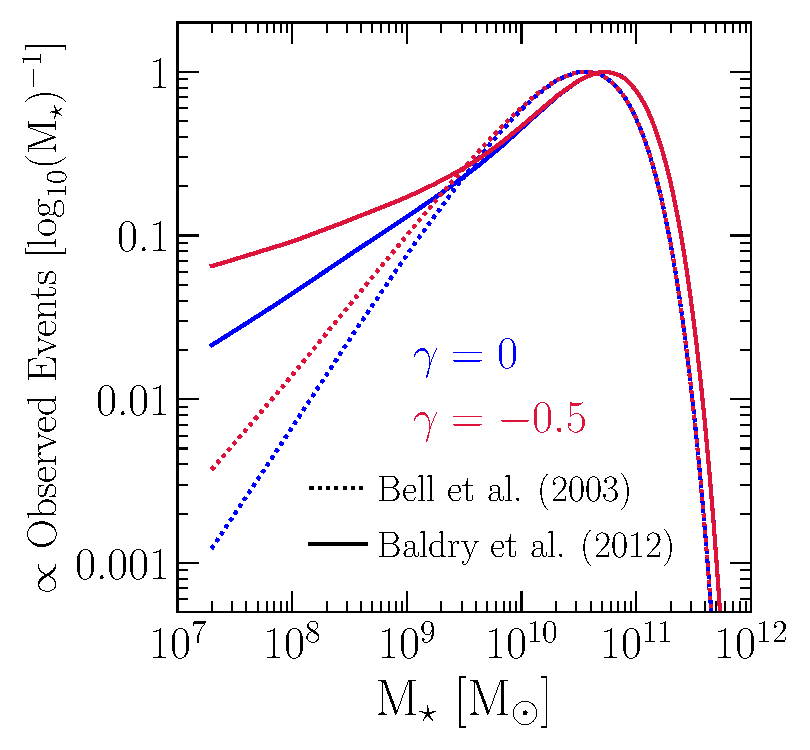
\includegraphics[scale = 0.55]{ia_massdist.pdf}
\caption{
The predicted stellar mass distribution of SN Ia host galaxies in an
untargeted survey (see equation~\ref{eq:hostmassdist}) with the
\citet[][dotted]{Bell2003} and~\citet[][solid]{Baldry2012} SMFs combined with
both metallicity-dependent ($\gamma = -0.5$, red) and metallicity-independent
rates ($\gamma = 0$, blue).
All distributions are normalized to a maximum value of 1.
}
\label{fig:hostmassdist}
\end{figure}

While empirical measurements of the specific SN Ia rate as a function of
stellar mass depend on the assumed SMF~\citep{Gandhi2022}, the host galaxy
mass distribution of observed events does not, making it a potentially more
observationally feasible diagnostic.
As noted in Fig.~\ref{fig:specia_metdep}, only dwarf galaxies are
significantly affected by a metallicity-dependent scaling of SN Ia rates due to
the shape of the MZR, so a~$\gamma \approx -0.5$ scaling should present as an
enhanced tail at the low-mass end of the distribution.
Although this empirical measurement does not depend on the SMF, our theoretical
prediction does because we must take into account the relative abundances of
galaxies of different stellar masses.
The observed rate in a bin of stellar mass can be expressed as the product
of the characteristic rate~$\dot{N}_\text{Ia}$ at a given stellar mass and
the integral of the SMF~$\Phi(M_\star)$ over the bin in stellar mass according
to
\begin{equation}
\dot{N}_\text{Ia,cosmic}(M_\star | \gamma) = \dot{N}_\text{Ia}(M_\star | \gamma)
\int_{M_\star}^{M_\star + dM_\star} \Phi(M_\star) dM_\star,
\label{eq:hostmassdist}
\end{equation}
where~$\dot{N}_\text{Ia}$ is given by the numerator of
equation~\refp{eq:specia}.
We plot this distribution in Fig.~\ref{fig:hostmassdist} for each combination
of~$\gamma = 0$ and~$-0.5$ with the SMFs parametrized by~\citet{Bell2003}
and~\citet{Baldry2012} in logarithmically spaced bins of stellar mass,
normalizing to a maximum value of 1 in all cases.
For untargeted surveys like ASAS-SN, equation~\refp{eq:hostmassdist} should
describe the observed host galaxy stellar mass distribution exactly, whereas
targeted surveys like the Lick Observatory SN Search~\citep[LOSS;][]{Li2000,
Filippenko2001} would be impacted by selection criteria.
\par
According to this formalism, galaxies with stellar masses of
$M_\star \approx 3-5 \times10^{10}~\msun$ should dominate the detected SN Ia
events for all choices of the SMF and~$\gamma$.
This peak arises as the optimal stellar mass which is high enough to produce a
large number of WDs, but being near the ``knee'' of the SMF, is not so high
that the galaxies themselves are rare.
For a given choice of the SMF, $\gamma = -0.5$ indeed enhances the low-mass
tail of the distribution, increasing the number of observed SN Ia events in
$M_\star \approx 10^{7.2}~\msun$ galaxies by a factor of~$\sim$3 relative to
$\gamma = 0$.
However, Fig.~\ref{fig:hostmassdist} indicates that this observed distribution
is a considerably better diagnostic of the SMF itself as opposed to the
metallicity dependence of SN Ia rates or lack thereof.
Between the position of the peak and~$10^{7.2}~\msun$, the host mass
distribution computed with the~\citet{Bell2003} SMF drops by~$\sim$2.5 orders
of magnitude while that computed with the~\citet{Baldry2012} SMF drops
by~$\sim$1.5 orders of magnitude.
Nonetheless, once precise knowledge of the SMF -- independent of SN rates -- is
available, this diagnostic could distinguish between different models for the
metallicity dependence of SN Ia rates.

\end{document}
